\documentclass[table]{beamer}

\usepackage[utf8]{inputenc}
\usepackage{enumitem}
\usepackage[font=small,labelfont=bf,labelformat=empty]{caption}


%\usetheme{Berlin}
%\usetheme{Antibes}
%\usetheme{Dresden}
%\usetheme{Ilmenau}
%\usetheme{Hannover}
\usetheme{Malmoe}

\usecolortheme{dove}
%\usefonttheme[onlylarge]{structurebold}
%http://www.hartwork.org/beamer-theme-matrix/

\renewcommand{\arraystretch}{1.5}

\title[Laser-Based Feature Extraction and Pattern Recognition in IMS]{Laser-Based Feature Extraction and Pattern Recognition in Intersection Management Systems}
\author{Gustavo Velasco-Hernández}
\institute[Universidad del Valle]
{
	
}
\date{Pattern Recognition, 2014}

\begin{document}

\frame{\titlepage}
\section*{Outline}

\frame{\tableofcontents}
\section{Introduction}

% ARQUITECTURA MULTISENSORIAL PARA UN SISTEMA DE MONITOREO Y SUPERVISIÓN DE UNA INTERSECCIÓN VEHICULAR
%\subsection{Context}
%\frame
%{
%	\frametitle{Context}
%	Master's Research Project:\\
%	Multisensor Architecture for a Vehicular Intersection Management System
%}
%\subsection{Problem Statement}
%\frame
%{
%	\frametitle{Transportation Systems}
%	Issues in traditional transportation systems
%	\begin{itemize}
%		\item[-] Congestion
%		\item[-] Traffic rules violation
%		\item[-] Vehicle interaction
%	\end{itemize}
%}

%\frame
%{
%	\frametitle{Transportation Systems}
%	Issues in traditional transportation systems
%	\begin{itemize}
%		\item[-] Congestion
%		\item[-] Traffic rules violation
%		\item[-] Vehicle interaction
%	\end{itemize}
%	Intersections are critical places in transportation systems
%}

%\frame
%{
%	\frametitle{Intelligent Transportation Systems}
%	Objectives of ITS
%	\begin{itemize}
%		\item[-] Increase safety
%		\item[-] Increase efficiency
%		\item[-] Reduce costs
%	\end{itemize}
%}

%\frame
%{
%	\frametitle{Intersection Management Systems}
%	Tasks
%	\begin{itemize}
%		\item[-] Traffic Monitoring
%		\item[-] Traffic Management
%		\item[-] Warning Advertisement
%	\end{itemize}
%}
%
%\frame
%{
%	\frametitle{Intersection Scenario}
%	\begin{itemize}
%		\item[-] Pedestrians, Vehicles (Cars, Two-wheeled vehicles, Big vehicles)
%		\item[-] Recognition, Classification, Tracking
%		\item[-] Incident detection, Intersection Management
%	\end{itemize}
%}
%\subsection{Objectives}
%
%\frame
%{
%	\frametitle{Objectives}
%	\begin{itemize}
%	\item Objectives
%		\begin{itemize}
%			\item Review of the state-of-the-art of sensor fusion in IMS
%			\item Techniques review and architecture design 
%			\item Laser and video sensor fusion implementation
%			\item Incident detection and warnings advertisement
%			\item Testing and Comparison
%		\end{itemize}
%	\item<2-> For the course project:
%		\begin{itemize}
%			\item<2-> In \textcolor{blue}{blue} are the tasks proposed for this course project.
%			\item<2-> In \textcolor{green}{green} are the tasks proposed as plus if time allows it.
%		\end{itemize}
%	\end{itemize}
%}
%\frame
%{
%	\frametitle{Objectives}
%	\begin{itemize}
%	\item Objectives
%		\begin{itemize}
%			\item \textcolor{blue}{Review of the state-of-the-art of Sensor Fusion in IMS}
%			\item \textcolor{blue}{Techniques review} \textcolor{green}{and architecture design}
%			\item \textcolor{blue}{Laser} \textcolor{green}{and video sensor fusion} \textcolor{blue}{implementation}
%			\item Incident detection and warnings advertisement
%			\item \textcolor{blue}{Testing and Comparison}
%		\end{itemize}
%	\item For the course project:
%		\begin{itemize}
%			\item In \textcolor{blue}{blue} are the tasks proposed for this course project.
%			\item In \textcolor{green}{green} are the tasks proposed as plus if time allows it.
%		\end{itemize}
%	\end{itemize}
%}
%
%\subsubsection{Review}
%\frame
%{
%	\frametitle{Objectives}
%	Objective 1. Review of the state-of-the-art of Sensor Fusion in IMS
%	\begin{itemize}
%		\item Intelligent Transportation Systems (ITS)
%		\item Intersection Management Systems (IMS)
%		\item Multisensor Data Fusion (MDF)
%		\item Laser-Video Data Fusion
%		\item IMS + LV-DF
%	\end{itemize}
%}
%
%\frame
%{
%	\frametitle{Objectives}
%	Objective 1. Review of the state-of-the-art of Sensor Fusion in IMS
%	\begin{itemize}
%		\item Intelligent Transportation Systems (ITS)
%		\item Intersection Management Systems (IMS)
%		\item \textcolor{blue}{\emph{Multisensor Data Fusion (MDF)}}
%		\item \textcolor{blue}{\emph{Laser-Video Data Fusion}}
%		\item \textcolor{blue}{\emph{IMS + LV-DF}}
%	\end{itemize}
%}
%\subsubsection{Techniques and Design}
%\frame
%{
%	\frametitle{Objectives}
%	Objective 2. Techniques review and architecture design
%	\begin{itemize}
%		\item Feature Extraction (Laser/Video)
%		\item Pattern Recognition (Laser/Video)
%		\item Classification (Laser/Video)
%		\item Decision (Laser/Video)
%		\item Low-Level, Mid-Level and High-Level Fusion
%	\end{itemize}
%}
%
%\frame
%{
%	\frametitle{Objectives}
%	Objective 2. Techniques review and architecture design
%	\begin{itemize}		
%		\item \textcolor{blue}{\emph{Feature Extraction (Laser}}\textcolor{green}{\emph{/Video)}}
%		\item \textcolor{blue}{\emph{Pattern Recognition (Laser}}\textcolor{green}{\emph{/Video)}}
%		\item \textcolor{green}{\emph{Classification (Laser/Video)}}
%		\item Decision (Laser/Video)
%		\item \textcolor{blue}{\emph{Low-Level, Mid-Level and High-Level Fusion}}
%	\end{itemize}
%}
%
%\subsubsection{Implementation}
%\frame
%{
%	\frametitle{Objectives}
%	Objective 3. Laser and video sensor fusion implementation
%	\begin{itemize}	
%		\item Implement choosen techniques for laser and video data
%		\item Integrate developed modules to the designed architecture for sensor fusion
%	\end{itemize}
%}
%
%\frame
%{
%	\frametitle{Objectives}
%	Objective 3. Laser and video sensor fusion implementation
%	\begin{itemize}	
%		\item \textcolor{blue}{\emph{Implement choosen techniques for laser}}\textcolor{green}{\emph{ and video data}}
%		\item \textcolor{green}{\emph{Integrate developed modules to the designed architecture for sensor fusion}}	
%	\end{itemize}
%}
%
%\subsubsection{Decision and Testing}
%\frame
%{
%	\begin{itemize}	
%		\item Objective 4. Incident detection and warnings advertisement
%		\item Objective 5. \textcolor{blue}{\emph{Testing and Comparison}}
%	\end{itemize}
%	
%	\emph{Objective 4 is out of the scope of this class.}
%}

%\subsection{Aims and Conditions}
\subsection{Aims}
\frame{
	\frametitle{Main Objective}
	- To develop a feature extraction and pattern recognition laser-based module for an intersection management system 
}
\frame{
	\frametitle{Sub-objectives}
	\begin{itemize}
		\item<1->[-] Review of laser-based feature extraction and pattern recognition in ITS and IMS
		\item<2->[-] Evaluate pros and cons of the reviewed methods
		\item<3->[-] Implement at least one method
		\item<4->[-] Evaluate implemented module and compare it with similar developments
	\end{itemize}
}
\subsection{Conditions}
\frame{
	\frametitle{Conditions}
	\begin{itemize}
		\item<1->[-] The information source will be a dataset.
		\item<2->[-] Just one laser.
	\end{itemize}
}

\subsection{Similar Projects}
%\frame
%{
%	\frametitle{Research Groups}
%	\begin{itemize}
%		\item[-] PKU Omni Smart Sensing (POSS) Research group at Peking University (POSS-i project)
%		\item[-] Institute of Measurement, Control and Microtechnology at Ulm University (Ko-PER program)
%		%Forschungsinitiative Ko-FAS from Bundesministerium für wirtschaft und Technologie (Germany)
%	\end{itemize}
%}
%
%\subsection*{POSS-i}
%\frame
%{
%	\frametitle{PKU Omni Smart Sensing (POSS)}
%	\begin{itemize}
%		\item[-] POSS is leaded by Prof. Huijing Zhao, Ph.D.
%		\item[-] Focus on perception technologies using an intelligent vehicle, a network sensing system or a collaboration of them
%	\end{itemize}
%}
%\frame
%{
%	\frametitle{POSS-i}	
%	\begin{figure}
%		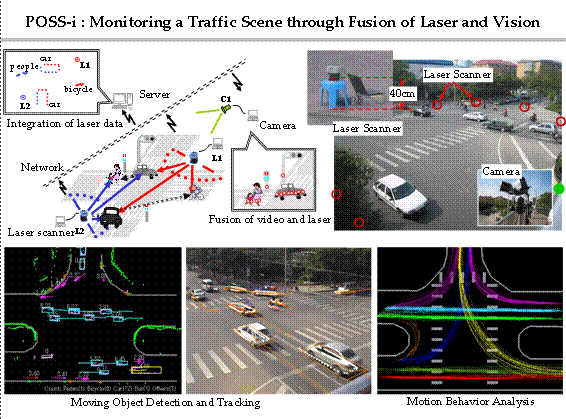
\includegraphics[scale=0.4]{fig/possi.png}
%		\caption{POSS-i project. [Zhao09][Zhao12][Song13b]}
%	\end{figure}
%}
%
%
%\subsection*{Ko-PER}
%\frame
%{
%	\frametitle{Ko-PER}
%	\begin{itemize}
%		\item[-] Ko-PER from Cooperative Perception
%		\item[-] Included in Forschungsinitiative Ko-FAS from Bundesministerium für wirtschaft und Technologie (Germany)
%		\item[-] Cooperative and collaborative sensors system for perception and preventive road safety.
%		\item[-] Daniel Meissen from Ulm University as leader researcher.
%	\end{itemize}
%}
%\frame
%{
%	\frametitle{Projects}	
%	\begin{figure}
%		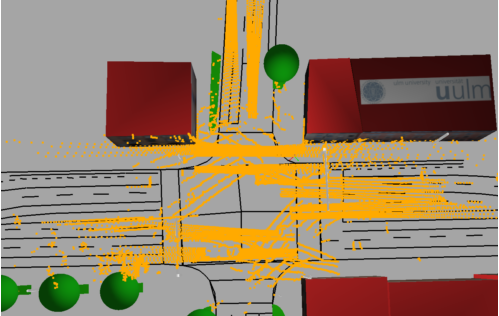
\includegraphics[scale=0.4]{fig/meiss1.png}
%		\caption{3D-recreated intersection scene with laser beams depicted [Meissner12, 13a, 13b, 13c, 14][Striegel13]}
%	\end{figure}
%}

\subsubsection*{Methods And Techniques}
\frame
{
	\frametitle{Applications, Methods and Techniques}
	
	\scriptsize{
	\begin{table}	
	\begin{tabular}{|c|c|c|}
	\hline
	Project & POSSi & Ko-PER \\
	\hline
	Applications & \multicolumn{2}{c|}{\parbox{6cm}{Recognition, Classification and Tracking of Vehicles and Pedestrians}} \\
	\hline
	\parbox{2.5cm}{Methods and \\Techniques}
	& \parbox{2.5cm}{\begin{itemize}[leftmargin=.07in]
		\item[-] Clustering
		\item[-] KL Transform
		\item[-] Markov Chains
		\item[-] Kalman Filtering
		\item[-] AdaBoost
	\end{itemize}
	}
	& \parbox{3.5cm}{
	\begin{itemize}[leftmargin=.07in]
		\item[-] DBSCAN
		\item[-] Multi-object Bayes Filter
		\item[-] Sequential Monte Carlo Methods
		\item[-] Dempster-Shafer Theory
		\item[-] Multiple-Model Probability Hypothesis Density Filter (in Gaussian Mixture representation)
	\end{itemize}
	}\\
	\hline
	
	\end{tabular}
	\caption{POSSi and PKU projects comparison}	
	\end{table}
	}
}

\frame
{
	\frametitle{Applications, Methods and Techniques}
	
	\scriptsize{
	\begin{table}	
	\begin{tabular}{|c|c|c|}
	\hline
	Project & POSSi & Ko-PER \\
	\hline
	Applications & \multicolumn{2}{c|}{\parbox{6cm}{Recognition, Classification and Tracking of Vehicles and Pedestrians}} \\
	\hline
	\parbox{2.5cm}{Methods and \\Techniques}
	& \parbox{2.5cm}{\begin{itemize}[leftmargin=.07in]
		\item[-] \textcolor{blue}{Clustering}
		\item[-] \textcolor{blue}{KL Transform}
		\item[-] \textcolor{blue}{Markov Chains}
		\item[-] Kalman Filtering
		\item[-] AdaBoost
	\end{itemize}
	}
	& \parbox{3.5cm}{
	\begin{itemize}[leftmargin=.07in]
		\item[-] \textcolor{blue}{DBSCAN}
		\item[-] Multi-object Bayes Filter
		\item[-] Sequential Monte Carlo Methods
		\item[-] Dempster-Shafer Theory
		\item[-] Multiple-Model Probability Hypothesis Density Filter (in Gaussian Mixture representation)
	\end{itemize}
	}\\
	\hline
	
	\end{tabular}
	\caption{POSSi and PKU projects comparison}	
	\end{table}
	}
}

\section{Solution Description}
\subsection{Introduction}
\frame{
	\frametitle{Typical System for one source of data}	
	\begin{figure}
		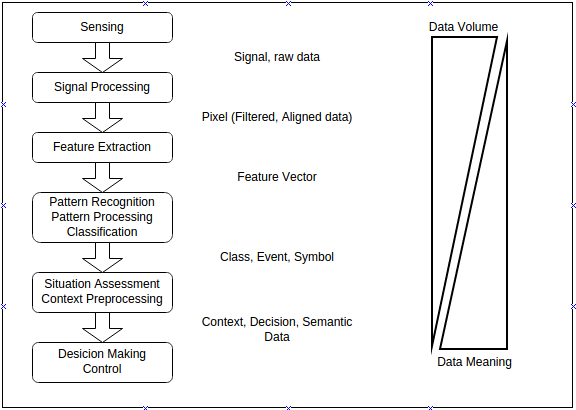
\includegraphics[scale=0.4]{fig/TypAppSys2.png}
		\caption{Single source system block diagram}
	\end{figure}
}
%\frame{
%	\frametitle{Multisensor Data System}	
%	\begin{figure}
%		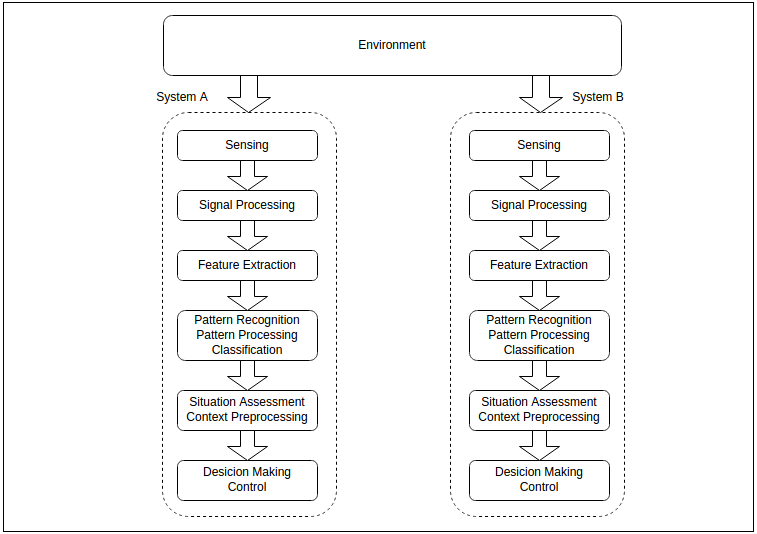
\includegraphics[scale=0.3]{fig/TypApp2.png}
%		\caption{Multisensor system block diagram}
%	\end{figure}
%}
%\frame{
%	\frametitle{How to fuse information?}	
%	\begin{figure}
%		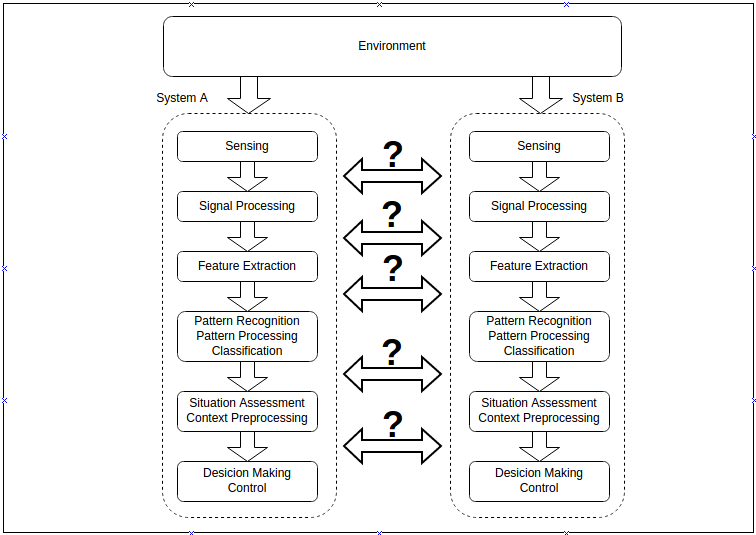
\includegraphics[scale=0.3]{fig/TypApp2q.png}
%		\caption{Multisensor system block diagram}
%	\end{figure}
%}
%\frame{
%	\frametitle{Fusion Levels}	
%	\begin{figure}
%		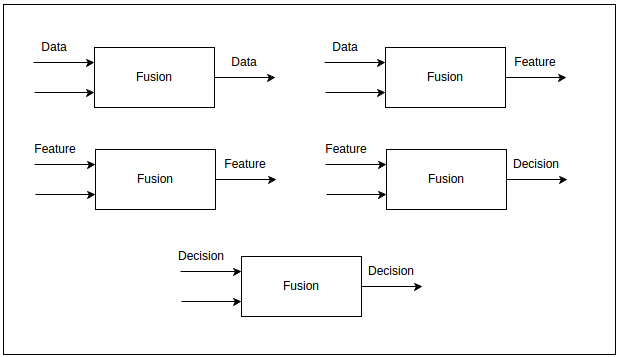
\includegraphics[scale=0.3]{fig/fusionLevels.png}
%		\caption{Fusion Levels [Luo11]}
%	\end{figure}
%}
%\frame{
%	\frametitle{Fusion Algorithms}	
%	\begin{figure}
%		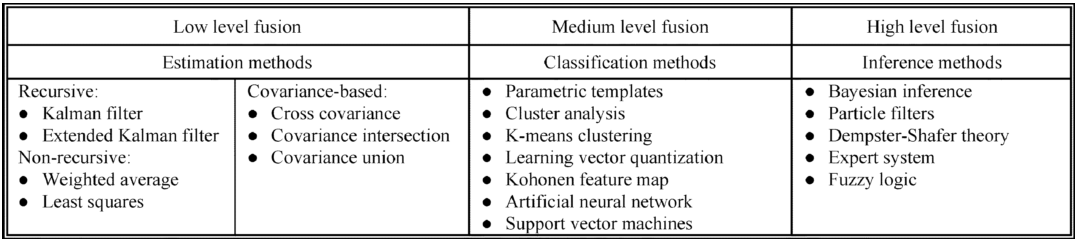
\includegraphics[scale=0.3]{fig/fusionAlg.png}
%		\caption{Classification of Fusion Algorithms [Luo11]}
%	\end{figure}
%}
%\subsection{Video Processing}
%\frame{
%	\frametitle{Video-Based System Block Diagram}
%	\begin{figure}
%		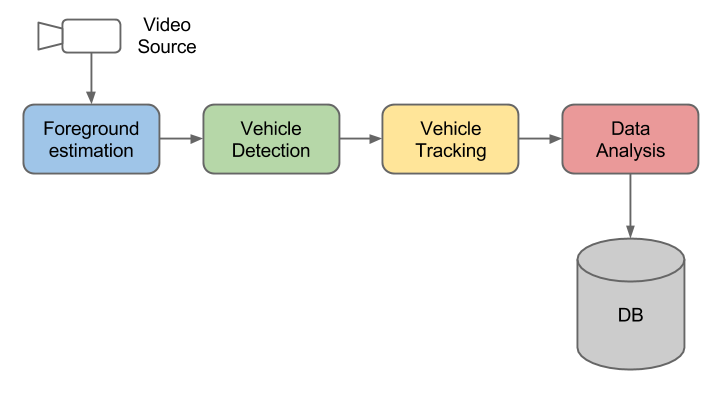
\includegraphics[scale=0.4]{fig/proposal1.png}
%	\end{figure}
%}
%\frame{
%	\frametitle{Video-Based System Block Diagram}
%	\begin{figure}
%		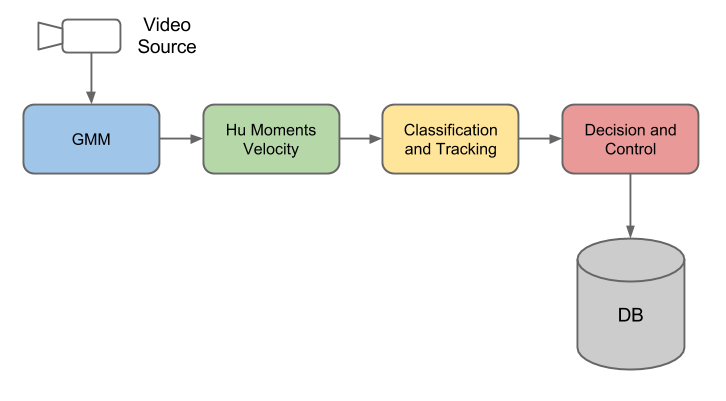
\includegraphics[scale=0.4]{fig/proposal1tech.png}
%	\end{figure}
%}
\subsection{Laser Processing}
\frame{
	\frametitle{Laser-Based System Block Diagram}
	\begin{figure}
		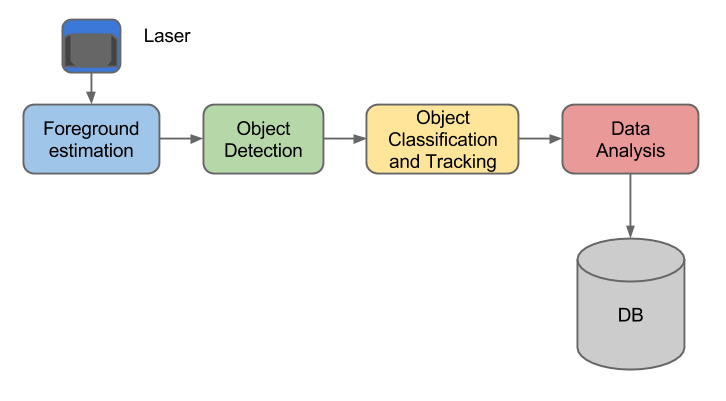
\includegraphics[scale=0.4]{fig/proposalLaser.png}
	\end{figure}
}
\frame{
	\frametitle{Laser-Based System Block Diagram}
	\begin{figure}
		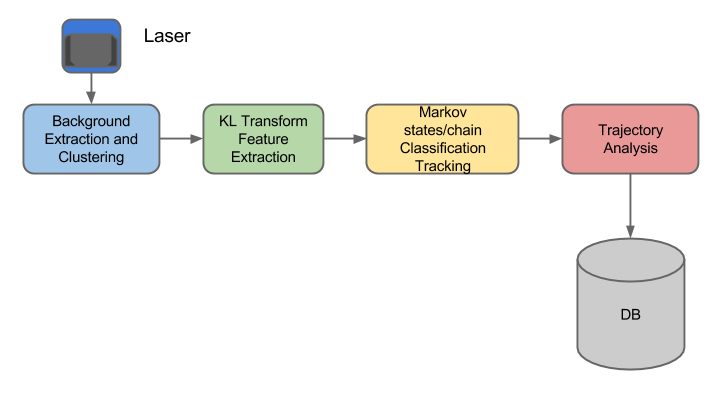
\includegraphics[scale=0.4]{fig/proposalLaserTech.png}
		\caption{Based on [Zhao06]}
	\end{figure}
}

\frame{
	\frametitle{System Description}
	\begin{figure}
		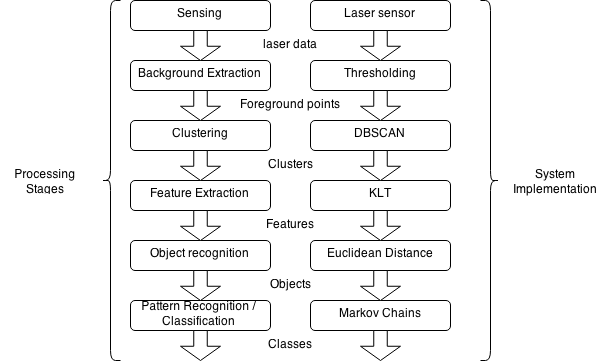
\includegraphics[scale=0.4]{fig/finalblockdiagram.png}
	\end{figure}
}

\section{Datasets and Implementation}

\subsection{Datasets Overview}

\frame{
	\frametitle{Dataset}
	\begin{itemize}
		\item[-] Although datasets for both projects are available, POSS-i dataset was choosen.
		\item[-] It includes laser readings from 6 laser-scanner located in different corners in an intersection.
		\item[-] The duration of scanning is approximately 10 minutes.
		%\item[-] A background model for each laser is provided
	\end{itemize}
}

\frame{
	\frametitle{Dataset}
	\begin{figure}
		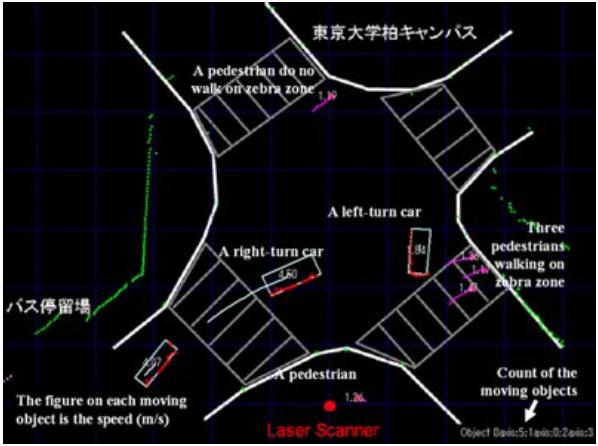
\includegraphics[scale=0.35]{fig/datasetview.png}
		\caption{Capture of dataset viewer application [Zhao06]}
	\end{figure}
}



\subsection{Foreground Estimation}
\frame{
	\frametitle{Background Extraction}
	\begin{itemize}
		\item[-] Histogram-based background extraction
		\item[-] Done for each angle
		\item[-] When a pick value is detected, tells that an object is detected
		\item<2->[\textcolor{green}{-}] \textcolor{green}{Dataset already includes a background model for each laser scanner}
	\end{itemize}
}

\frame{
	\frametitle{Clustering}
	\begin{itemize}
		\item[-] In [Zhao06] it is not detailed how clustering was done, so DBSCAN is proposed to identify clusters in laser-data points
	\end{itemize}
}

\frame{
	\frametitle{DBSCAN - Introduction}
	\begin{itemize}
		\item[-] Density-Based Spatial Clustering for Applications with Noise
		\item[-] Proposed by Ester et al in 1996 in KDD conference [Ester96].
	\end{itemize}
}

\frame{
	\frametitle{DBSCAN - Explanation}
	\begin{itemize}
		\item[-] The algorithm needs two parameters: $Eps (\epsilon)$ and $minPts$
		\item[-] Also are defined two types of points: Core points and border points
		\item[-] $p$ is a core point if in its $Eps$-$Neighborhood$ are at least $minPts$ points.
	\end{itemize}
	\begin{figure}
		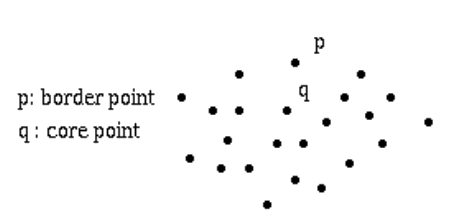
\includegraphics[scale=0.35]{fig/cbpoints.png}
		\scriptsize{\caption{Types of points [Ester96]}}
	\end{figure}
}

\frame{
	\frametitle{DBSCAN - Algorithm}
	\begin{itemize}
		\item[-] DBSCAN starts at an arbitrary point $p$, then evaluate if point's $Eps$-$Neighnorhood$ contains at least $minPts$ points
		\item[-] If $True$, $p$ is a core point (Is in a cluster)
		\begin{itemize}
			\item[-] Assign $clusterId$ to p and its neighbour, and neighbours of its neighbours and so on.
			\item[-] Increase $clusterId$.		
		\end{itemize}
		\item[-] If $False$, $p$ is labelled as Noise
		\item[-] Continue with an unlabelled point, until all points in dataset are labelled.
	\end{itemize}
}

\frame
{
	\frametitle{Clustering}
	\begin{figure}
		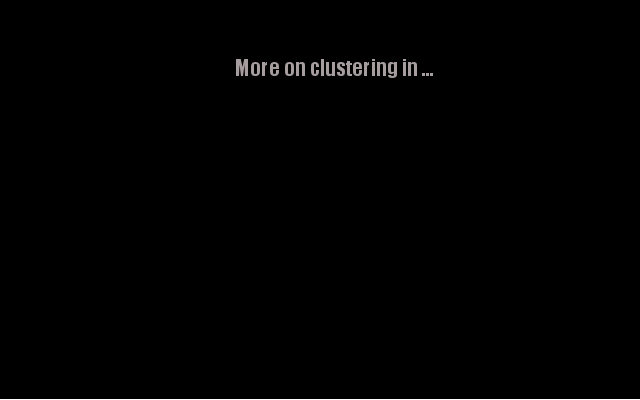
\includegraphics[scale=0.45]{fig/ulcs1.png}		
	\end{figure}
}
\frame
{
	\frametitle{Clustering}
	\begin{figure}
		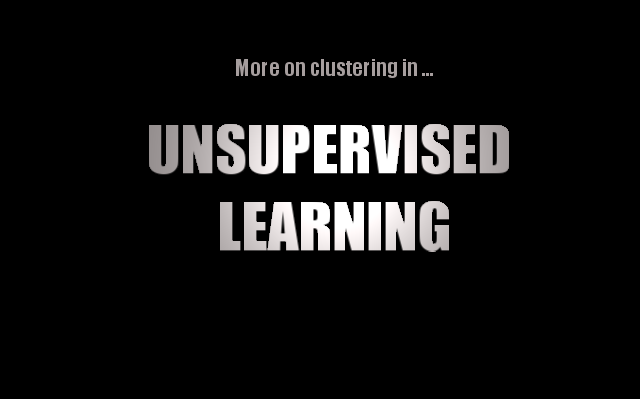
\includegraphics[scale=0.45]{fig/ulcs2.png}	
	\end{figure}
}
\frame
{
	\frametitle{Clustering}
	\begin{figure}
		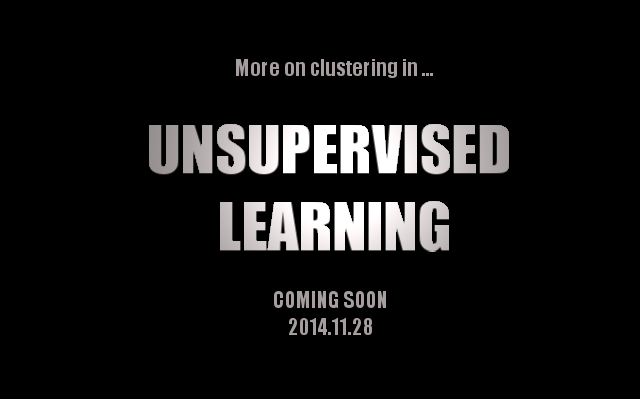
\includegraphics[scale=0.45]{fig/ulcs3.png}	
	\end{figure}
}

\subsection{Feature Extraction and Classification}
\frame{
	\frametitle{Definitions}
	\begin{itemize}
		\item[-] Classes are proposed based on distribution of points in clusters
		\item[-] Karhunen-Loeve Transform to detect number of axis
		\begin{figure}
			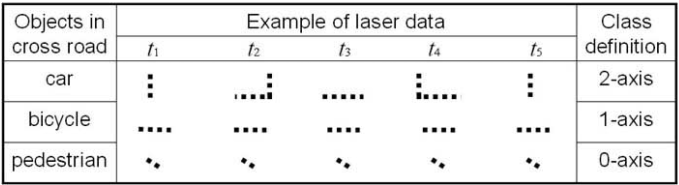
\includegraphics[scale=0.4]{fig/objClasses.png}
		\end{figure}
	\end{itemize}
}
\frame{
	\frametitle{Markov States}
		\begin{figure}
			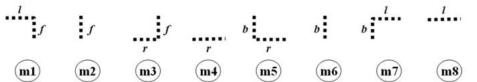
\includegraphics[scale=0.4]{fig/mstates.png}
			\caption{There are 8 patterns that can happen}
			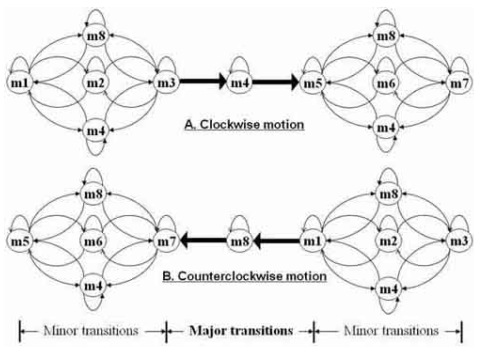
\includegraphics[scale=0.3]{fig/mtrans.png}
			\caption{Possible transitions}
		\end{figure}
}

\frame{
	\frametitle{Features}
	\begin{itemize}
		\item[-] Normal Vectors
		\item[-] Number of axis
		\item[-] Axis lengths		
		\item[-] Directional vector, Motion speed
		\item[-] Markov States		
	\end{itemize}
}
\frame{
	\frametitle{Classification and Tracking}
	\begin{itemize}
		\item[-] Classification and tracking stages are under review
	\end{itemize}
}

\subsection{Next Steps}
\frame{
	\frametitle{Next Steps}
	\begin{itemize}
		\item[-] Implement Dataset handler
		\item[-] Implement Clustering and KL Transform to classify in 0, 1 or 2 axis object
		\item[-] Get features from objects and obtain trajectory
	\end{itemize}
}

%\frame{
%	\frametitle{Definition}
%	\begin{columns}[c] % the "c" option specifies center vertical alignment
%    \column{.5\textwidth} % column designated by a command
%    		\begin{figure}
%		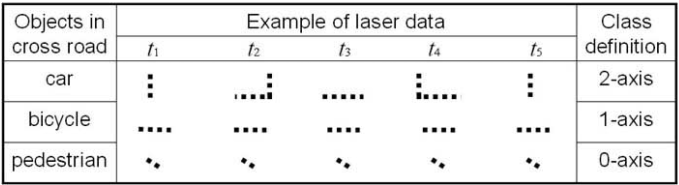
\includegraphics[scale=0.2]{fig/objClasses.png}
%	\end{figure}
%    \column{.5\textwidth}
%     Contents split \\ into two lines
%    \end{columns}
%}

%\frame{
%	\frametitle{Conditions}
%	\begin{itemize}
%		\item<1-> The video source will be a file or dataset.
%		\item<2-> Daylight and good weather (no rain, no fog, no snow).
%	\end{itemize}

%}
%
%\section{Initial Solution Proposal}
%\frame{
%	\frametitle{Block Diagram}
%	\begin{figure}
%		%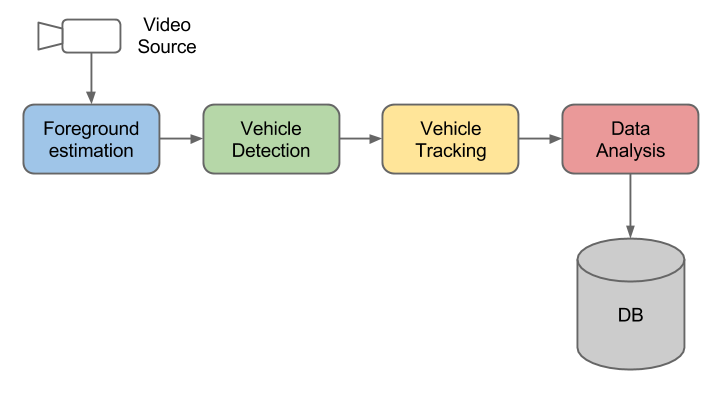
\includegraphics[scale=0.4]{fig/proposal1.png}
%	\end{figure}
%}
%\subsection{Foreground Estimation}
%\frame{
%	\frametitle{Foreground Estimation}
%	\begin{figure}
%		%\includegraphics[scale=0.4]{fig/fgall.png}
%	\end{figure}
%}
%\frame{
%	\frametitle{Foreground Estimation}
%	\begin{figure}
%		%\includegraphics[scale=0.4]{fig/fgsel.png}
%	\end{figure}
%}
%
%\subsection{Vehicle Detection}
%\frame{
%	\frametitle{Vehicle Detection}
%	\begin{figure}
%		%\includegraphics[scale=0.3]{fig/vdall.png}
%	\end{figure}
%}
%\frame{
%	\frametitle{Vehicle Detection}
%	\begin{figure}
%		%\includegraphics[scale=0.4]{fig/vdsel.png}
%	\end{figure}
%}
%
%\subsection{Vehicle Tracking}
%\frame{
%	\frametitle{Vehicle Tracking}
%	\begin{figure}
%		%\includegraphics[scale=0.4]{fig/vtall.png}
%	\end{figure}
%}
%
%\frame{
%	\frametitle{Vehicle Tracking}
%	\begin{figure}
%		%\includegraphics[scale=0.4]{fig/vtsel.png}
%	\end{figure}
%}
%
%
%\section{Methods and Techniques}
%\subsection{Foreground Estimation}
%\frame{
%	\frametitle{Gaussian Distribution}
%	\begin{itemize}
%	
%	\item<1-> Univariate\\
%	\[	p(x) = \frac{1}{{\sigma \sqrt {2\pi } }}e^{{-\frac{1}{2}}{{\frac{(x-\mu)^2 }{\sigma ^2 }}}}=\mathcal{N}(x;\mu,\sigma^2)\] 
%	\item<2-> Multivariate (N)\\
%	\[
%	p(x) = {(2\pi)^{\frac{N}{2}}}{\left|\Sigma\right|}^{-\frac{1}{2}}e^{({-\frac{1}{2}}{{{(\boldsymbol{x}-\boldsymbol{\mu})^T}{\Sigma^{-1}}{(\boldsymbol{x}-\boldsymbol{\mu})}}})}=\mathcal{N}(\boldsymbol{x};\boldsymbol{\mu},\Sigma)
%	\]
%	\[dim(\boldsymbol{x})= 1 x N\]
%	\[dim(\boldsymbol{\mu})= 1 x N\]
%	\[dim(\Sigma)= N x N\]
%	
%	\end{itemize}
%	
%}
%\frame{
%	\frametitle{Gaussian Distribution}
%	\begin{figure}
%		%\includegraphics[scale=0.7]{fig/gaussians.eps}
%		\caption{Univariate and Multivariate Gaussians (Chuong B. Do, \textit{The Multivariate Gaussian Distribution}, 2008.)}
%	\end{figure}
%}
%\frame{
%	\frametitle{Gaussian Mixture Model}
%	\[z \in \{g_1,g_2,...,g_k\}\]\\
%	\[p(x) = \displaystyle\sum_{i=1}^{k}{p(x\mid z)p(z)}= \displaystyle\sum_{i=1}^{k}{p(x\mid z=g_i)p(z=g_i)}\]\\
%	\[p(x) = \displaystyle\sum_{i=1}^{k}{\alpha_i \mathcal{N}(x;\boldsymbol{\mu}_i,\Sigma_i)}\]\\
%	
%}
%\frame{
%	\frametitle{Expectation-Maximization Algorithm}
%	\[p(x) = \displaystyle\sum_{n=1}^{K}{\alpha_k \mathcal{N}(x;\boldsymbol{\mu}_k,\Sigma_k)}\]\\
%	\begin{itemize}
%		\item E-step: Assume we know $\pi_i, \mu_i, \Sigma_i$\\
%		\[ e_{ij} = \pi_i{(2\pi)^{\frac{N}{2}}}{\left|\Sigma\right|}^{-\frac{1}{2}}e^{({-\frac{1}{2}}{{{(\boldsymbol{x_i}-\boldsymbol{\mu_i})^T}{\Sigma^{-1}}{(\boldsymbol{x_i}-\boldsymbol{\mu_i})}}})}\]		
%	\end{itemize}
%}
%\frame{
%	\frametitle{Expectation-Maximization Algorithm}
%	\begin{itemize}
%	\item M-step: Update Values\\
%		\[ \pi_i = \displaystyle\sum_{j}\frac{e_{ij}}{M}\]
%		\[ \mu_i = \displaystyle\sum_{j}\frac{e_{ij}x_{ij}}{M}\]
%		\[ \Sigma_i = \frac{\displaystyle\sum_{j}e_{ij}(x_j - \mu_j)^T(x_j-\mu_j)}{\displaystyle\sum_{j}e_{ij}}\]
%	\end{itemize}
%}
%\frame{
%	\frametitle{Expectation-Maximization Example}
%	\begin{figure}
%		%\includegraphics[scale=0.37]{fig/EMiterations4.png}
%		\caption{Iterations 1,3,5,20 of EM Algorithm (Andrew W. Moore, \textit{Clustering with Gaussian Mixtures},2004)}
%	\end{figure}
%}
%
%\subsection{Vehicle Detection}
%\frame
%{
%	\frametitle{Countour Based Approach [Buch08]}
%
%	Detection
%	\begin{itemize}
%		\item Find closed contours on foreground mask
%		\item Calculate overlap of a contour's area with the ROI
%		\item Get valid silhouettes
%	\end{itemize}
%}
%
%\frame
%{
%	\frametitle{Countour Based Approach [Buch08]}
%
%	$\{S_m\}$: Closed contours\\
%	$L(S_m)$: Length of contour\\
%	$A()$: Area operator\\
%	$O(S_m,R) \in {0,1}$: Overlap operator\\
%	$\tau_L$: Lenght threshold\\
%	$\tau_O$: Overlap threshold\\
%	
%	\[O(S_m,R) = \frac{A(S_m \bigcap R)}{A(S_m)}\]
%	
%	\[S_k = \{ S_m \mid L(S_m) > \tau_L \wedge O(S_m,R) > \tau_O\}\]
%}
%
%\frame
%{
%	\frametitle{Countour Based Approach}
%
%	Classification
%	\begin{itemize}
%		\item Get silhouettes from detection stage
%		\item Generate 3D hypothesis from silhoutte
%		\item Generate model masks for each hypothesis and project it on the image
%		\item Find the best fit of the model masks. 
%	\end{itemize}
%}
%
%\frame
%{
%	\frametitle{Models used by [Buch08]}
%
%	\begin{figure}
%		%\includegraphics[scale=0.1]{fig/models_plain.jpg}
%		\caption{Wire frame models used for classification}
%	\end{figure}
%}
%
%\frame
%{
%	\frametitle{Implementation}
%
%	\begin{itemize}
%		\item Get all contours
%		\item Filter by length and areas
%	\end{itemize}
%}
%
%\subsection{Tracking}
%\frame
%{
%	\frametitle{Moments calculation}
%
%	\begin{itemize}
%		\item Calculate moments and get center of mass for each valid contour
%		\[x = \frac{m_{01}}{m_{00}}; y = \frac{m_{10}}{m_{00}}\]
%		\item Find similar in previous detected
%		\item If found similar contour, update it  and append new center of mass.
%		\item If not found, store it
%	\end{itemize}
%}
%
%\frame
%{
%	\frametitle{Tracking}
%
%	\begin{itemize}
%		\item An object's path is defined by center of mass history.
%		\item An intersection area was defined, so a valid object should appear and disappear outside of it.	
%		\item An object is considered inactive when leaves the intersection.
%		
%	\end{itemize}
%}
%
%\section{Similar Projects}
%\frame
%{
%	\frametitle{An Improved Adaptive Gaussian Mixture Model For Real-time Tracking and Shadow Detection. \textit{KaewTraKulPong, 2004}}
%
%	Features
%	\begin{itemize}
%		\item Mixture of K gaussians
%		\item Online EM algorithm (Use L-recent window)
%		\item Shadow detection option		
%	\end{itemize}
%}
%
%\frame
%{
%	\frametitle{Improved Adaptive Gaussian Mixture Model for Background Subtraction.	\textit{Zivkovic, 2004}}
%
%	Features
%	\begin{itemize}
%		\item Mixture of K gaussians (K-adaptive)
%		\item Online EM algorithm (Use L-recent window)
%	\end{itemize}
%}
%
%\frame
%{
%	\frametitle{Algorithm}
%	
%	Each pixel is modeled with a mixture of K gaussians, using h recent values.
%	
%	\begin{itemize}
%		\item Parameters: History length (h), varThreshold(v)
%		\item Online EM algorithm
%		\item K dynamically generated
%	\end{itemize}	
%}
%
%\frame
%{
%	\frametitle{Algorithm}
%	\begin{itemize}
%		\item Parameters: History length (h), varThreshold(v)
%		\item Online EM algorithm
%		\item K dynamically generated
%	\end{itemize}	
%}
%
%\frame
%{
%	\frametitle{Algorithm}
%	\begin{itemize}
%		\item Last h values are used to generate the K-GMM
%		\item Mahalanobis distance from the components to the sample is calculated to estimate which is the closer.
%		\item If there is no 'close' component, a new one is created with 
%		\[\pi = \alpha, \mu = x, \sigma = \sigma_0\]
%	\end{itemize}	
%}
%
%\section{Results}
%
%\frame
%{
%	\frametitle{Dataset}
%	\begin{figure}
%		%\includegraphics[scale=0.1]{fig/dataset_beijing.jpg}
%		\caption{Video capture from Zhao et al, 2009.}
%	\end{figure}
%}
%\subsection{Foreground Estimation}
%\frame
%{
%	\frametitle{History Length comparison}
%	\begin{figure}
%		%\includegraphics[scale=0.1]{fig/history_comparison.jpg}
%		\caption{Frame 4380 with v=9 and h=[300, 500, 700]}
%	\end{figure}
%}
%
%\frame
%{
%	\frametitle{History Length comparison}
%	\begin{figure}
%		%\includegraphics[scale=0.1]{fig/history_comparison2.jpg}
%		\caption{Frame 2260 with v=9 and h= [300, 500, 700]}
%	\end{figure}
%}
%
%\frame
%{
%	\frametitle{Threshold comparison}
%	\begin{figure}
%		%\includegraphics[scale=0.1]{fig/v_2260_h500.jpg}
%		\caption{Frame 2260 with h=500 and v= [9, 21, 45]}
%	\end{figure}
%}
%
%\frame
%{
%	\frametitle{Threshold comparison}
%	\begin{figure}
%		%\includegraphics[scale=0.1]{fig/varT_comparison2.jpg}
%		\caption{Frame 6390 with h=700 and v= [9, 21, 45]}
%	\end{figure}
%}
%
%\frame
%{
%	\frametitle{Foreground estimation}
%	\begin{figure}
%		%\includegraphics[scale=0.1]{fig/results123.jpg}
%		\caption{Estimated foreground of frames 2160, 2260, 4380 using h = 500 and v=21}
%	\end{figure}
%}
%
%\frame
%{
%	\frametitle{Foreground estimation}
%	\begin{figure}
%		%\includegraphics[scale=0.15]{fig/results45.jpg}
%		\caption{Estimated foreground of frames 6170 and 6390 using h = 500 and v=21}
%	\end{figure}
%}
%
%\frame
%{
%	\frametitle{Shadows?}
%	\begin{figure}
%		%\includegraphics[scale=0.15]{fig/shadows.jpg}
%		\caption{Shadow detection: Disabled and Enabled}
%	\end{figure}
%}
%\subsection{Vehicle detection}
%\frame
%{
%	\frametitle{Contour detection results}
%	\begin{figure}
%		%\includegraphics[scale=0.1]{fig/contours.jpg}
%		\caption{Contours detected}
%	\end{figure}
%}
%
%\subsection{Tracking}
%\frame
%{
%	\frametitle{Tracking results}
%	\begin{figure}
%		%\includegraphics[scale=0.1]{fig/tracking.jpg}
%		\caption{Frames showing objects detected and their paths}
%	\end{figure}
%}
%
%\subsection{Summary}
%\frame
%{
%	\frametitle{Processing time}
%	Processing time (min/avg/max) [ms]
%	\begin{itemize}
%		\item Foreground Extraction: 72.62/83.71/180.97 ms
%		\item Total: 89.41/120.97/257.72 ms
%	\end{itemize}
%	
%}
%
\section{References}
\subsection{References}
\frame
{
	\frametitle{References}
	\footnotesize{	
	\begin{itemize}[leftmargin=.6in]
		\item [Elmenreich07] Elmenreich, W. \textbf{A Review on System Architectures for Sensor Fusion Applications}. \textit{Software Technologies for Embedded and Ubiquitous Systems
Lecture Notes in Computer Science Volume 4761 (pp. 547–559)}. 2007.
		\item [Esteban12] Esteban, J. et al, \textbf{A Review of data fusion models and architectures: towards 	engineering guidelines}. \textit{Neural Computing and Applications, 14(4),(pp. 273–281)}. 2012.
		\item [Ester96] Ester, M. et al. \textbf{A Density-Based Algorithm for Discovering Clusters in Large Spatial Databases with Noise}. \textit{Proceedings of 2nd International Conference on Knowledge Discovery and Data Mining (KDD-96)}. 1996.
		\item [Goldhammer12] Goldhammer, M. et al, \textbf{Cooperative multi sensor network for traffic safety applications at intersections}. \textit{2012 15th International IEEE Conference on Intelligent Transportation Systems (pp. 1178–1183)}. 2012.		
	\end{itemize}
	}
}

\frame
{
	\frametitle{References}
	\footnotesize{	
	\begin{itemize}[leftmargin=.6in]
		\item [Khaleghi11] Khaleghi, B. et al, \textbf{Multisensor data fusion: A review of the state-of-the-art}. \textit{Information Fusion, 14(1) (pp. 28–44)}. 2011.
		\item [Luo02] Luo, R. C. \textbf{Multisensor fusion and integration: approaches, applications, and future research directions}. \textit{IEEE Sensors Journal, 2(2), 107–119}. 2002
		\item [Luo11] Luo, R. C. et al. \textbf{Multisensor Fusion and Integration: Theories, Applications, and its Perspectives}. \textit{IEEE Sensors Journal, 11(12), 3122–3138}. 2011.
	    \item [Meissner10] Meissner, D. and Dietmayer, K. \textbf{Simulation and calibration of infrastructure based laser scanner networks at intersections}.\textit{2010 IEEE Intelligent Vehicles Symposium, 670–675}. 2010.	    
	\end{itemize}
	}
}

\frame
{
	\frametitle{References}
		\footnotesize{
	\begin{itemize}[leftmargin=.6in]
		\item [Meissner12] Meissner, D., Reuter, S., and Dietmayer, K. \textbf{Real-time detection and tracking of pedestrians at intersections using a network of laserscanners}. \textit{2012 IEEE Intelligent Vehicles Symposium, 630–635}. 2012.
		\item [Meissner13a] Meissner, D., Reuter, S., and Dietmayer, K. \textbf{Road user tracking at intersections using a multiple-model PHD filter}. \textit{2013 IEEE Intelligent Vehicles Symposium (IV), (Iv), 377–382}. 2013.
		\item [Meissner13b] Meissner, D. et al. \textbf{Road User Tracking Using a Dempster-Shafer Based Classifying Multiple-Model PHD Filter}. \textit{Information Fusion (FUSION), 2013 16th International Conference on (Vol. 32, pp. 1236–1242)} 2013.
		\item [Meissner13c] Meissner, D., Reuter, S., and Dietmayer, K. \textbf{Combining the 2D and 3D world: a new approach for point cloud based object detection}. \textit{IET Intelligent Signal Processing Conference 2013 (ISP 2013) (pp. 4.1–4.1)}. 2013.				
	\end{itemize}	
	}
}

\frame
{
	\frametitle{References}
		\footnotesize{
	\begin{itemize}[leftmargin=.6in]
		\item [Meissner14] Meissner, D. et al. \textbf{Intersection-Based Road User Tracking Using a Classifying Multiple-Model PHD Filter}.\textit{ IEEE Intelligent Transportation Systems Magazine, 6(April 2014), 21–33}.2014.
		\item [Song08] Song, X. et al. \textbf{Bayesian fusion of laser and vision for multiple People Detection and tracking}. \textit{2008 SICE Annual Conference, 3014–3019}. 2008.
		\item [Song13a] Song, X. et al. \textbf{Laser-based tracking of multiple interacting pedestrians via on-line learning}. \textit{Neurocomputing, 115, 92–105}. 2013.
		\item [Song13b] Song,X. et al. \textbf{An Online System for Multiple Interacting Targets Tracking: Fusion of Laser and Vision, Tracking and Learning}. \textit{ACM Transactions on Intelligent Systems and Technology}. 2013.		
	\end{itemize}	
	}
}

\frame
{
	\frametitle{References}
		\footnotesize{
	\begin{itemize}[leftmargin=.6in]
		\item [Strigel13] Strigel, E., Meissner, D., and Dietmayer, K. \textbf{Vehicle detection and tracking at intersections by fusing multiple camera views}. \textit{2013 IEEE Intelligent Vehicles Symposium (IV) (pp. 882–887)}. 2013.
		\item [Zhao06] Zhao, H., and Shibasaki, R. \textbf{Joint tracking and classification of moving objects at intersection using a single-row laser range scanner}. \textit{In Proceedings of the IEEE Intelligent Transportation Systems Conference (pp. 287–294)}. 2006.
		\item [Zhao08] Zhao, H. et al.\textbf{ Monitoring an intersection using a network of laser scanners}. \textit{Proceedings of the11th International IEEE Conference on Intelligent Transportation Systems (pp. 428–433)}. 2008.
		\item [Zhao09] Zhao, H., Cui, J., and Zha, H. \textbf{Sensing an Intersection Using a Network of Laser Scanners and Video Cameras}. \textit{IEEE Intelligent Transportation Systems Magazine, 31–37}. 2009.
		\item [Zhao12] Zhao, H. et al. \textbf{Detection and Tracking of Moving Objects at Intersections Using a Network of Laser Scanners}. \textit{IEEE Transactions on Intelligent Transportation Systems, 13(2), 1–16}. 2012.

	\end{itemize}	
	}
}

%\frame
%{
%	\frametitle{References}
%		\footnotesize{
%	\begin{itemize}[leftmargin=.6in]
%
%
%	\end{itemize}	
%	}
%}
% BIBENTRY TEMPLATE
%\item [Goldhammer12] Goldhammer, M. et al, \textbf{Cooperative multi sensor network for traffic safety applications at intersections}. \textit{2012 15th International IEEE Conference on Intelligent Transportation Systems (pp. 1178–1183)}. 2012.

%
%
%

%
%
%
%
%\item [Chuong08] Chuong B. Do, \textit{The Multivariate Gaussian Distribution}, 2008.
%		\item [Moore04] Andrew W. Moore, \textit{Clustering with Gaussian Mixtures},2004.
%		\item [Kaew04] KaewTraKulPong et al, \textit{An Improved Adaptive Gaussian Mixture Model For Real-time Tracking and Shadow Detection}, 2004.
%		\item [Zhao09] Zhao, H. et al, \textit{Sensing an intersection using a network of laser scanners and video cameras}, IEEE Intelligent Transportation Systems Magazine, vol.1, no.2, 31-37, 2009.
%		\item [Buck08] Buch, N et al \textit{Detection and Classification of vehicles for urban traffic scene}, 2008

\end{document}
